\chapter{Система имитационного моделирования.}

\section{Архитектура подсистемы имитационного моделирования}

В данном разделе будет рассмотрена работа подсистемы имитационного моделирования производственных процессов (\ref{ris:arh1}). 
Работа имитационной модели состоит из следующих этапов:

\begin{enumerate}
    \item[\mylabel{itm:point1}{1})] Создание шаблона продукта. Шаблон представляет из себя структуру данных, являющуюся технологической картой одной единицы конкретного продукта. 
	\item[\mylabel{itm:point2}{2})] Создание ЦПВ. ЦПВ представляет из себя список структур данных, включающим в себя шаблон и необходимое количество продукта.
	\item[\mylabel{itm:point3}{3})] Следующим этапом является развертывание единого плана на основе заказа. Производственный план описывает совокупность операций\footnote{Так как технологическая карта описывается набором операций, а заказ описывается перечнем технологических карт и их количеством, появилась возможность описать план совокупностью операций.} и состояние ресурсов.
    \item[\mylabel{itm:point4}{4})] Пошаговая расчет плана с учетом ресурсных ограничений, где каждый раз при расчете переменной из системы неравенств, обновляется информации о состоянии ресурсов.
\end{enumerate}

Работа имитационного моделирования представлена на рисунке \ref{ris:alg}
\begin{figure}[H]
    \center{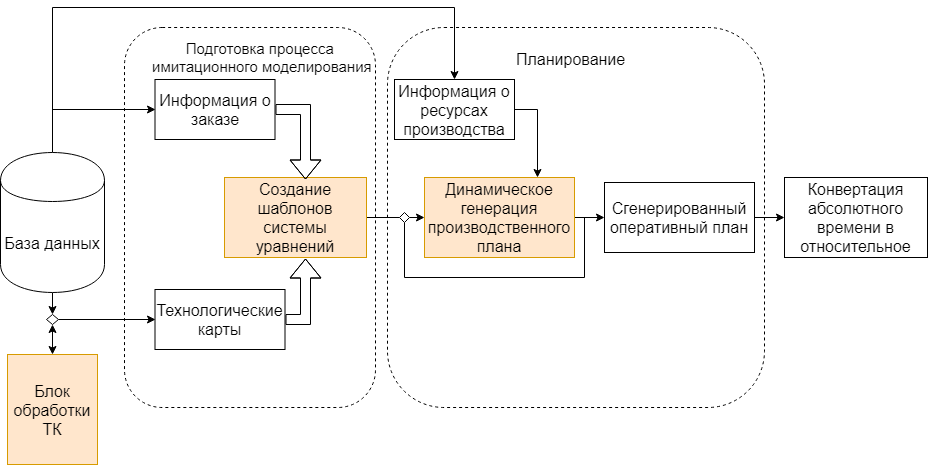
\includegraphics[width=1\linewidth]{fig/alg_2.png}}
    \caption{Визуализация работы имитационного моделирования}
    \label{ris:alg}
\end{figure}

\section{Входные и выходные данные}

\subsection{Входные данные}
В данном разделе приведена структура входных данных для имитационной модели.

\begin{itemize}
	\item ЦПВ - цеховая последовательность выпуска (выпуск продукции осуществляется в порядке, в котором они записаны в ЦПВ):
		\begin{itemize}
			\item[а)] наименование продукции;
			\item[б)] количество единиц продукции;	
			\item[в)] технологическая карта.
		\end{itemize}			
	\item Технологические карты, подробнее смотри (\ref{assembly_line_balancing:input_data}).
	\item Производственные ресурсы;
	\item \textit{Трафик доступности ресурсов};
	\item \textit{Структура цеха};
	\item \textit{Минимальное время участия ресурса в операции};
	\item \textit{Штрафы за переключение ресурса с одной операции на другую}. 
\end{itemize}

\subsection{Выходные данные}

\begin{itemize}
	\item Расчетные данные:	
		\begin{itemize}
			\item[а)] перечень всех операций для всех единиц продукции ЦПВ;
			\item[б)] время начала всех операций;
			\item[в)] время окончания всех операций;
			\item[г)] \textit{производственные ресурсы, привлекаемые к выполнению операции};
			\item[д)] \textit{время начала и конца участия ресурса в операции};
			\item[е)] \textit{загрузка производственных ресурсов}.
		\end{itemize}		
	\item Визуализация данных пользователю:
		\begin{itemize}
			\item[а)] расписания для производственных ресурсов;
			\item[б)] диаграммы Ганта выпуска разных видов продукции;
			\item[в)] визуализация загрузки производственных ресурсов.
		\end{itemize}		 
\end{itemize}

\section{Этапы имитационного моделирования}
В данном разделе подробно описаны все этапы имитационного моделирования.
На изображении (\ref{ris:DataFlow}) приведена диаграмма потоков данных.

\begin{figure}[H]
    \center{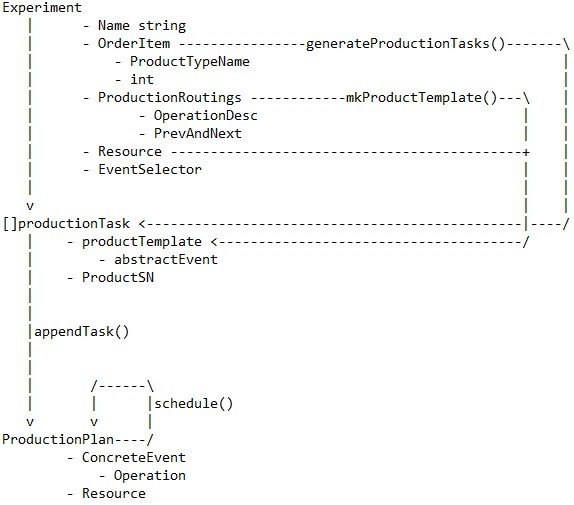
\includegraphics[width=1\linewidth]{fig/MkExperimentDataFLow.jpg}}
    \caption{Диаграмма потоков данных}
    \label{ris:DataFlow}
\end{figure}

\subsection{Предобработка технологических карт}

\subsubsection*{Входные данные}
\indent Входными данными для данного элемента ПО является технологическая карта с конфигурациями ресурсов\footnote{Примером конфигурации ресурса может являться вычисление длительности операции на основе количества персонала, привязанного к операции.}. 

\subsubsection*{Выходные данные}
Выходными данными являются технологическая карта с зафиксированными значениями.

\subsubsection*{Процесс предобработки}
\label{prepeocess}
Одним из первых этапов работы алгоритма имитационного моделирования является подготовка входных данных, полученных из базы данных. 

На текущий момент реализована функционал отвечающий за предварительную обработку. Одной из таких функций является расчет длительности операций. Так как длительность операций является переменной величиной, зависимой от трудоемкости и количества людей выполняющих операцию, существует четыре настройки ресурса:

\begin{enumerate}
    \item[1)] минимальная, при этом на операцию назначается минимальное количество людей, длительность операции становится максимальной;
    \item[2)] максимальная, при этом на операцию назначается максимальное количество людей, длительность операции становится минимальной;
    \item[3)] средняя при этом на операцию назначается среднее количество людей, длительность операции становится средней;
    \item[4)] случайная, при этом количество персонала на операцию выбирается случайным образом. 
\end{enumerate}

Также к предварительной настройке относится алгоритм выбора операции\footnote{В тех случаях, когда на этапе планирования есть независимые операции}. На данный момент существует две конфигурации:

\begin{itemize}
    \item[1)] стандартная, при которой выбор осуществляется строго по порядку расположения в структурах данных;
    \item[2)] случайная, при этом случайным образом выбирается одна из возможных операций, которые доступны в данный момент. 
\end{itemize}

Возможность менять входные данные является важным этапом обработки входных данных полученных из базы данных, позволяя при этом подготовить данные для дальнейшей обработки, а также гибко менять параметризуемые величины, чем и достигается большая вариативность необходимая для поиска оптимального значения.

Реализацию функции предобработки технологических карт представлена в Приложении А, Листинг 1.

\subsection{Создание шаблона продукта}

\subsubsection*{Входные данные}
Входными данными для данного элемента имитационной модели является технологическая карта с фиксированными значениями (прошедшая обработку после базы данных).

\subsubsection*{Выходные данные}
\label{imcore:mkProductTemplate_output_data}
Выходными данными является структура данных, включающая в себя набор событий и привязок ресурсов к каждому событию.

\subsubsection*{Описание реализации}
Как говорилось ранее, любая технологическая карта состоит из перечня операций. В процессе работы было принято решение разделить операцию на события, это было вызвано удобством представления аналитических уравнений.

Основной задачей процесса создания шаблона продукта является подготовка необходимых структур данных для дальнейшей работы имитационной модели. На диаграмме потоков данных \ref{ris:DataFlow}, данный процесс именуется как - mkProductTemplate(). В результате работы mkProductTemplate(), создается шаблон продукта необходимый для структуры описывающий заказ.

Реализация функции создания шаблона технологической карты представлена в Приложении А, Листинг 2.

\subsection{Создание заказа}

\subsubsection*{Входные данные}
Входными данными является перечень продуктов и количество каждого продукта из этого перечня.

\label{imcore:generateProductionTasks_output_data}

\subsubsection*{Выходные данные}
Выходными данными является список структур описываемых в разделе \ref{imcore:mkProductTemplate_output_data}, то есть шаблон и количество данного продукта.

\subsubsection*{Описание реализации}
На диаграмме потоков данных \ref{ris:DataFlow} процесс создания заказа называется - generateProductionTasks(). Основной задачей функции заказа является генерация шаблонов продуктов в зависимости от их количества, при этом каждый однотипный шаблон имеет уникальный идентификатор (серийный номер).

Реализация функции создания заказа представлена в Приложении А, Листинг 3.


\subsection{Планирование}

\subsubsection*{Входные данные}
Входными данными для функции планирования является производственное задание на одну единицу продукции, полученное из списка сформировавшемся на этапе создания заказа (\ref{imcore:generateProductionTasks_output_data}).

\subsubsection*{Выходные данные}
Выходными данными является производственный план, состоящий из событий, операций и состояния ресурсов.

\subsubsection*{Описание реализации}
Основной задачей этапа планирования заключается в составлении плана, согласно которому выполняется привязка каждой операции для каждой единицы продукции к временным интервалам, конкретному работнику и конкретным производственным средствам. На диаграмме потоков данных \ref{ris:DataFlow} процесс отвечающий за создание задания на одну единицу продукции называется appendTask(). Задание включает в себя шаблон технологической карты, название продукта, а также его серийный номер. Процесс формирования заданий работает до тех пор, пока не учтёт всю информацию из полученного заказа. Следующим этапом является процесс планирования на диаграмме потоков данных \ref{ris:DataFlow} данный процесс называется – schedule(). Именно на данном этапе в работу включается модель ресурсов, описываемая далее в разделе \ref{resource}. Основными особенностями данного этапа является сопоставление требованиям ресурсов к операциям, к ресурсным возможностям предприятия, от того строится реальный план, учитывающий ресурсные ограничения. 

Результирующая блок-схема подсистемы имитационного моделирования изображена на рисунке \ref{ris:IM_blockShema}.

\begin{figure}[H]
    \center{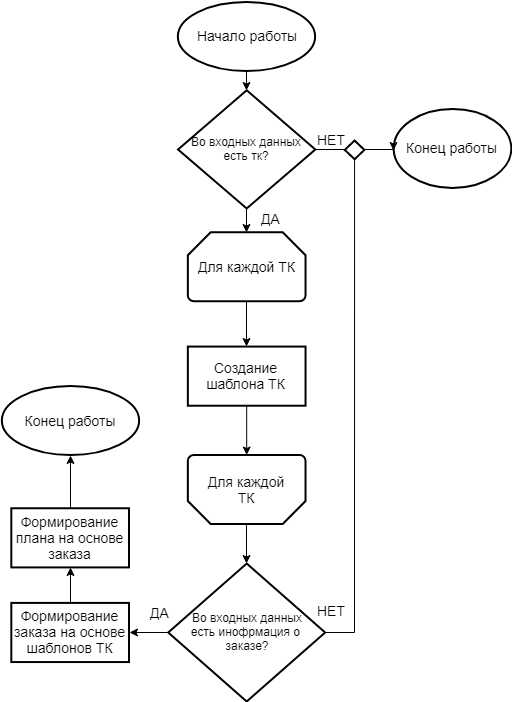
\includegraphics[scale=0.55]{fig/BlockShemaImcore.png}}
    \caption{Схема работы имитационного моделирования}
    \label{ris:IM_blockShema}
\end{figure}

Реализация алгоритма планирования представлена в Приложении В, Листинг 4,5.

\subsection{Алгоритм модели ресурсов}
\label{resource}

\indent В процессе создания оперативного плана, для получения корректной оценки времени выполнения операции или набора операций СПП необходимо ввести систему ограничений, которая будет отражать как ресурс, участвующий в операции может влиять на её время выполнения.
Это привело к созданию модели ресурсов накладывающей ограничения на выбор операции для расчета ядром имитационного моделирования.
Под ресурсом подразумевается любое устройство,деталь,инструмент или средство,за исключением сырьевого материала и промежуточного продукта, находящиеся в распоряжении предприятия для производства товаров и услуг.
В соответствии с данным определением к ресурсам относятся в том числе и человеческие ресурсы, которые в данной системе не рассматриваются с точки зрения поведения или других аспектов человеческой жизни, а лишь с точки зрения возможности выполнить конкретную задачу.
Также необходимо обозначить, что в данном разделе под моделью ресурса будет пониматься упрощенная модель реального ресурса, отражающая его основные (в рамках выполняемых операций) характеристики.\\
\indent Каждая модель ресурса представляет из себя структуру данных, которая должна реализовывать три метода (Листинг 3.1):
\begin{itemize}
	\item метод привязки операции к модели ресурса;
	\item метод, осуществляющий проверку возможности выполнения данной операции моделью ресурса;
	\item метод, осуществляющий логику работы и в котором происходит изменение состояния данной модели.
\end{itemize}

\begin{lstlisting}[language=Golang,caption={Описание методов ресурса},label=lst:code]
	type Resource interface {
		Bind(conf interface{}, events ...*ConcreteEvent)
		Constrain(event *ConcreteEvent) (int64, bool)
		Done(event *ConcreteEvent)
		Clone() Resource
	}
\end{lstlisting}

\indent Под привязкой операции к модели подразумевается добавление операции в очередь на выполнение и, если это первая привязанная для данного продукта операция, то добавление продукта в очередь на распределение. Привязка осуществляется в начале работы системы, что позволяет ресурсам манипулировать ядром имитационного моделирования разрешая или запрещая выбирать привязанные к ним операции для расчета, что может повлечь за собой изменение последовательности выполнения операций и, соответственно, расчетного времени выполнения карты технологического процесса.

\begin{figure}[h]
	\centering
	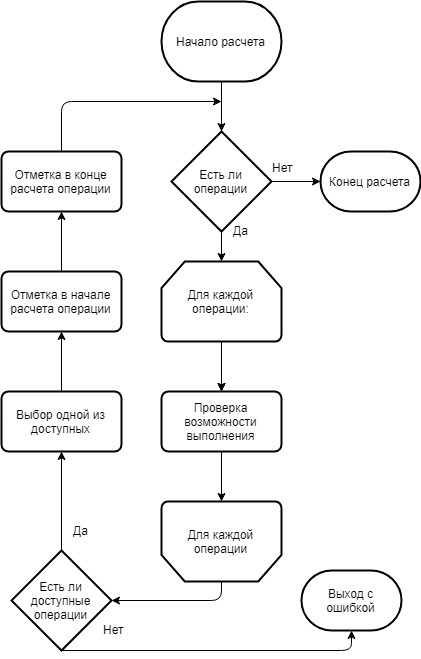
\includegraphics[scale=0.6]{fig/assemblyResSchema.png}
	\caption{Схема работы ядра моделирования с ресурсами в процессе расчета оперативного плана}
	\label{fig:assemblyResSchema}
\end{figure}

\indent Проверка производится во время работы системы и именно здесь происходит отбор операций в соответствии с внутренним состоянием модели.\\
\indent Логика осуществляется при выборке операции ядром и для каждой вызывается два раза: чтобы отметить состояние модели в начале и в конце расчета операции (см. \ref{fig:assemblyResSchema}).


% СПП имеет несколько видов ресурса, одним из которых является модель ресурса рабочих. Задача данной модели заключается в учете занятости каждого работника. Для упрощения работы модели было принято объединить группы работников одной
Одной из реализованных моделей ресурсов является модель рабочих. В предыдущем разделе уже было сказано, что ресурс рабочих рассматривается с точки зрения необходимого элемента функционирования предприятия, при этом упускаются особенности жизнедеятельности рабочих. Это ведет к тому, что на текущий момент не введены соответствующие погрешности регулирующие различные ситуации\footnote{Cостояние работника, внеплановые перерывы и т.д.}, что соответствующим образом уменьшает точность модели. 

В данной работе ресурс работника характеризуется общим количеством работников данной профессии (квалификации). Также в виде структуры данных реализовано состояние ресурса, которое включает следующие элементы:

\begin{itemize}
	\item операции, которые предстоит выполнить рабочим; 
	\item операции, которые уже выполнены;
	\item количество людей данной профессии на конкретную операцию, конкретного продукта, включая серийный номер;
	\item привязку каждого конкретного работника к выполняемой операции;
	\item последний временная метка, на которой остановились работы;
	\item карта занятости рабочих, смотри рисунок \ref{ris:Staff}.
\end{itemize}

Карта занятости является основным источником информации для системы распределения ресурсов. Как видно из данной карты, первые три операции выполнялись строго последовательно, четвертая независимая от предыдущих была определена системой в самое начало последовательности операций. Таким образом первая и четвертая операция будут выполнены одновременно. Решение о том переносе четвертой операции было принято исходя из следующих факторов. Во первый данная операция не связанна с предыдущими причинно – следственными связями. Во-вторых, есть необходимое число свободных работников на данном промежутке времени.

\begin{figure}[H]
    \center{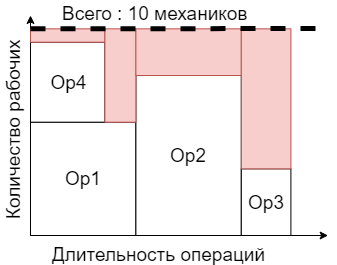
\includegraphics[scale = 0.5]{fig/Staff.png}}
    \caption{Карта занятости рабочих}
    \label{ris:Staff}
\end{figure}

Может показаться, что информация, описывающая состояние ресурса избыточна, но это не так, потому что не все перечисленные выше элементы участвуют в логике ресурса. Некоторые элементы, такие как привязки каждого конкретного работника к выполняемой операции, используется для расчёта объемно календарного планирования.


\subsection{Оптимизация на уровне имитационного моделирования}

Как упоминалось ранее, в разделе посвященном предобработке технологической карты \ref{prepeocess}, исходная ТК предполагает вариативность конфигурации, отсюда следует, что потенциально имитационная модель может сгенерировать большое количество разных оперативных планов.

На рисунке \ref{ris:IM_process} приведена зависимость сгенерированного оперативного плана от выбранного критерия оптимальности.


\begin{figure}[H]
    \center{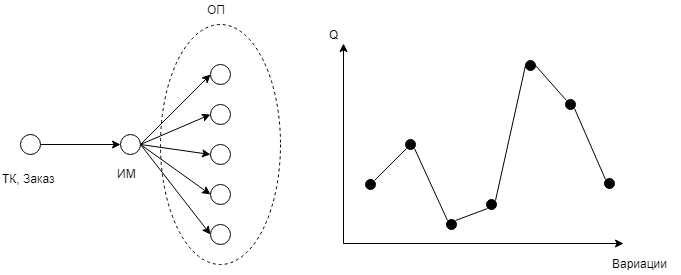
\includegraphics[scale = 0.6]{fig/IM_process.png}}
    \caption{Процесс формирования оперативных планов и оценка их качества}
    \label{ris:IM_process}
\end{figure}

В следующем разделе приведены методы, которые позволяют подсистеме оптимизации (рис.\ref{ris:optimization}) на уровне имитационной модели, найти оптимальную последовательность операций. Критерием оптимальности в данном случае является минимальное время работы линии.

\begin{figure}[H]
    \center{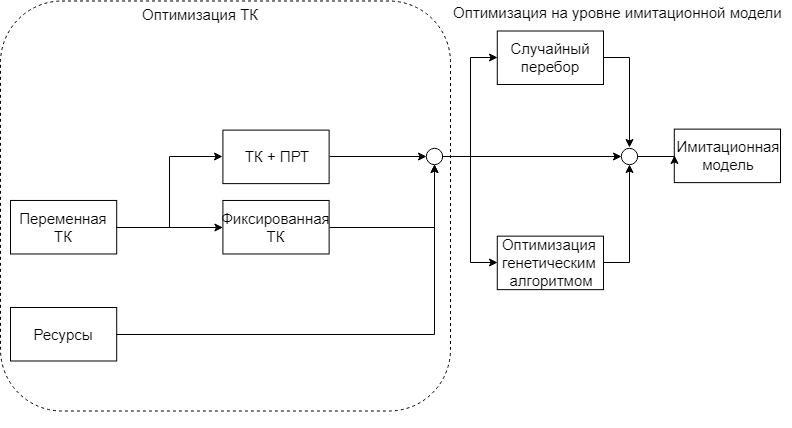
\includegraphics[width=1\linewidth]{fig/Opt.png}}
    \caption{Подсистема оптимизации}
    \label{ris:optimization}
\end{figure}


\subsubsection*{Метод случайного перебора}
Оптимизация на уровне имитационной модели работает непосредственно в процессе планирования, при этом основная задача оптимизации сводится к выбору наиболее «правильной» операции, которая будет выбрана следующей в формировании последовательности операций. Таким образом можно говорить о построении оптимальный последовательности операций, которая учитывает равномерную загрузку ресурсов, а также минимизацию времени работы над заготовкой. На рисунке \ref{ris:Force} изображены технологическая карта продукта и два плана, который были построены в результате случайного выбора операций.

\begin{figure}[H]
    \center{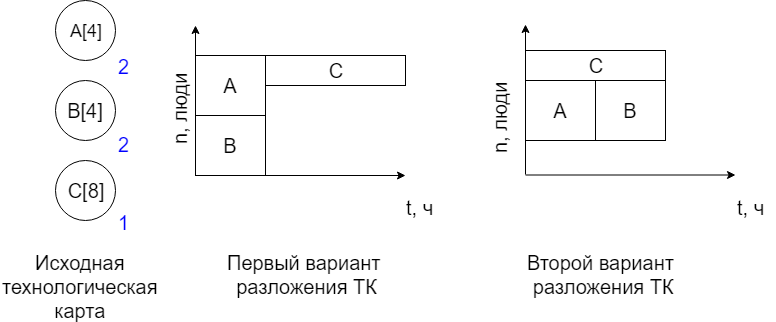
\includegraphics[width=1\linewidth]{fig/DecompositionOfTk.png}}
    \caption{Два плана, полученные путем перебора исходной технологической карты}
    \label{ris:Force}
\end{figure}

Пример на рисунке \ref{ris:Force} демонстрирует, то что при комбинировании операций достигается разный результат. При этом стоит отметить, что от выбранного критерия оптимальности, зависит и конечный результат. Так можно заметить корреляцию между равномерной загрузкой рабочих ресурсов и длительностью выполнения работ, которая отражается в том, что равномерное распределение задач среди рабочих ведет и к уменьшению общей длительности работы.

\subsubsection*{Генетические алгоритмы}
Основной задачей данного подхода является поиск оптимального значения путем смешивания и введения небольших правок (мутаций) в выборку наилучших решений.
Идеей такого рода алгоритмов является направленность поиска, которая позволяет преодолеть плато решений, при которых не происходит изменений в лучшую сторону. 


\section*{Эксперименты эффективности оптимизации}
\label{experiment}
Результаты экспериментов показали, что эффективность оптимизации во многом зависит от размера и состава входных данных.

Так на входных данных полученных от реального производства, оптимизация случайным перебором показала себя не эффективно. В первую очередь это связано с размером входных данных\footnote{325 операций в одной технологической карте.}. В вторых это связано со сложностью алгоритма планирования, так как сам случайный перебор является его частью, что делает его зависимым от реализации имитационной модели.

Также стоит отметить проблемы, связанные с входными данными. Данные проблемы заключаются в вариативности данных. На уровне имитационной модели метод случайного перебора может оперировать только выбором следующей операции на обработку. Таким образом, если операции на выбор только одна, в случае когда последовательность операций в технологической карте задана строгим образом и такая связь задана для большинства операций, то количество вариантов стремится к минимуму, а значит и целесообразность применения метода ставится под вопросом.

В результате эксперимента была сделаны следующие выводы. Метод случайного перебора зависит от размера входных данных, при этом важно оценивать входные данные на предмет вариативности. В том числе стоит отметить, что сложность задачи определяется пользователем на этапе конфигурации перебора\footnote{Имеется ввиду количество созданных планов со случайной последовательностью операций.}, что еще сильнее повышает ценность предварительной оценки технологической карты, с целью оценки надобности алгоритма перебора.

\section{Результаты работы имитационной модели}

Проведение экспериментов над имитационной моделью показали следующие результаты.

Во первых при большом объеме входных данных имитационная модель не растет экспоненциально. Данный факт подтверждается проведенными экспериментами. Соответствующий график приведен на рисунке \ref{ris:Computational_complexity_imcore}.
Более того, из данного графика видно, что рост сложности линеен.
% Данная проблема частично решилась благодаря использованию возможностей языка программирования golang, при этом задача имитационного моделирования разделась на потоки, что позволяло одновременно обрабатывать несколько входных технологических карт.

\begin{figure}[H]
    \center{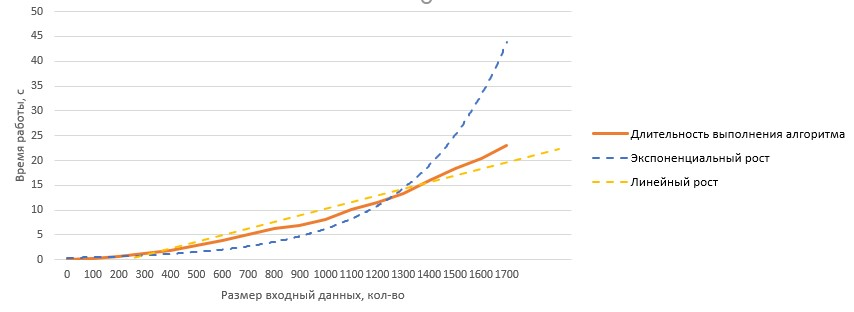
\includegraphics[width=1\linewidth]{fig/Computational_complexity_imcore.jpg}}
    \caption{Временная сложность имитационной модели}
    \label{ris:Computational_complexity_imcore}
\end{figure}

Далее приведен график временной сложности расчета оперативного плана для конвейеризированного производства. Данный график приведен на рисунке \ref{ris:Computational_complexity_assembly}. Как и в предыдущем случае модель показала линейный рост, но стоит отметить большее время расчета по сравнению с обычным планированием при одинаковом размере входных данных.

\begin{figure}[H]
    \center{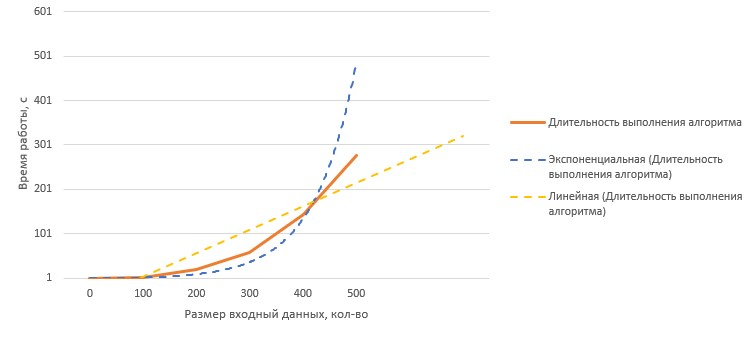
\includegraphics[width=1\linewidth]{fig/Computational_complexity_assembly.jpg}}
    \caption{Временная сложность имитационной модели конвейеризированного производства}
    \label{ris:Computational_complexity_assembly}
\end{figure}

Также была исследована разница между параллельным и последовательным расчетом имитационной модели. Были получены следующие результаты, представленные на рисунке \ref{ris:Parallellllee}. Данный эксперимент был проведен при 100, 500 и 1000 запусков планирования. Таким образом видно насколько эффективно справляется со своими задачами параллелизм реализованный в Golang.

\begin{figure}[H]
    \center{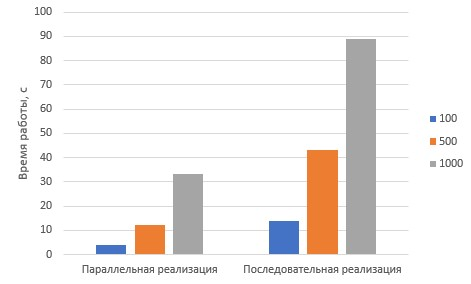
\includegraphics[scale = 0.9]{fig/Parallellllee.jpg}}
    \caption{Параллельный и последовательный расчет имитационной модели}
    \label{ris:Parallellllee}
\end{figure}

Во вторых выяснилось, что потенциально основной проблемой в будущем может оказаться сбор реальных данных для работы имитационной модели.
В рамках дипломной работы проверка имитационной модели проверялась на реальных технологических картах, при этом возник закономерный вопрос о сложности получения и организации данных о предприятии. 

